
%(BEGIN_QUESTION)
% Copyright 2010, Tony R. Kuphaldt, released under the Creative Commons Attribution License (v 1.0)
% This means you may do almost anything with this work of mine, so long as you give me proper credit

Read and outline the ``Relating I/O Status to Virtual Elements'' subsection of the ``Logic Programming'' section of the ``Programmable Logic Controllers'' chapter in your {\it Lessons In Industrial Instrumentation} textbook.  Note the page numbers where important illustrations, photographs, equations, tables, and other relevant details are found.  Prepare to thoughtfully discuss with your instructor and classmates the concepts and examples explored in this reading.

\vskip 10pt

The fundamental concept of relating I/O status to program elements is not necessarily easy to grasp.  For this reason, a ``Process Switches and PLC Circuits'' worksheet has been placed in the {\it Socratic Instrumentation} practice worksheet collection.  Feel free to use this practice worksheet to supplement your studies on this critically important topic!

\underbar{file i04516}
%(END_QUESTION)





%(BEGIN_ANSWER)


%(END_ANSWER)





%(BEGIN_NOTES)


\begin{itemize}
\item{} {\bf Each input bit in the PLC's memory will be a ``1'' when its input channel is powered, and will be a ``0'' when its input channel is unpowered}
\vskip 5pt
\item{} {\bf Each virtual contact shown in the program {\it actuates} whenever it reads a ``1'' state in its respective bit, and will be {\it at rest} whenever it reads a ``0'' state in its respective bit}
\vskip 5pt
\item{} {\bf A colored contact is {\it closed} (passes virtual power in the PLC program), while an un-colored contact is {\it open} (blocks virtual power in the PLC program)}
\end{itemize}

$$\includegraphics[width=15.5cm]{i04516x04.eps}$$

An input bit in a PLC's memory is set to 1 when it is electrically energized.  De-energized input bits are cleared to a value of 0.  Therefore, any PLC program contact whose real-world input is de-energized will be in its resting state.

A chain of causation exists from real-world input energization to contact coloring: energization causes bit state, which in turn causes virtual contact actuation, which in turn causes colorization (virtual continuity).

\vskip 10pt

PLC program coil colorization works similar: a colored coil writes a 1 to the output bit, turning that channel on.  An un-colored coil writes a 0 to the output bit, turning that channel off.

\vskip 10pt

In the high-pressure alarm system, the PLC performs a ``latching'' function using a seal-in contact {\tt Y5} to keep the alarm lamp energized even after the high-pressure event passes.








\vfil \eject

\vskip 20pt \vbox{\hrule \hbox{\strut \vrule{} {\bf Suggestions for Socratic discussion} \vrule} \hrule}

\begin{itemize}
\item{} Challenge students to identify input bit states for any of the illustrations in the book by convering up the portion of the diagram showing the I/O lamp statuses and switch states, and only showing students the ``live'' program view.
\item{} For each of the common misconceptions listed in the book, provide a practical example where that misconception is proven to be false.
\item{} Explain the functioning of the pressure alarm system PLC program through each step of the system's operation (pressure high, pressure low, reset button pressed, etc.).
\item{} Explain why it makes sense to label a virtual contact instruction (in the pressure alarm system) with an {\it output} bit address ({\tt Y5}).
\item{} Examining the high-pressure alarm PLC system shown near the end of this section, identify the effects of the Reset switch failing shorted.
\item{} Examining the high-pressure alarm PLC system shown near the end of this section, identify the effects of the Pressure switch failing open.
\end{itemize}













\vfil \eject

\noindent
{\bf Prep Quiz:}

Suppose two momentary-contact switches are connected to separate input channels of a PLC -- a normally-open switch connected to input X3 and another normally-open switch connected to input X5.  Given the following program running in the PLC, determine the states of output channels Y1 and Y2 with neither pushbutton pressed:

$$\includegraphics[width=15.5cm]{i04516x01.eps}$$

\vfil \eject

\noindent
{\bf Prep Quiz:}

Suppose two momentary-contact switches are connected to separate input channels of a PLC -- a normally-open switch connected to input X3 and another normally-open switch connected to input X5.  Given the following program running in the PLC, determine the states of output channels Y1 and Y2 with neither pushbutton pressed:

$$\includegraphics[width=15.5cm]{i04516x02.eps}$$

\vfil \eject

\noindent
{\bf Prep Quiz:}

Suppose two momentary-contact switches are connected to separate input channels of a PLC -- a normally-open switch connected to input X3 and another normally-open switch connected to input X5.  Given the following program running in the PLC, determine the states of output channels Y1 and Y2 with neither pushbutton pressed:

$$\includegraphics[width=15.5cm]{i04516x03.eps}$$


%INDEX% Reading assignment: Lessons In Industrial Instrumentation, Programmable Logic Controllers (relating I/O status to virtual elements)

%(END_NOTES)

